\documentclass[14pt]{beamer}
\usepackage{./Estilos/BeamerUVM}
\usepackage{./Estilos/ColoresLatex}
\usetheme{Madrid}
\usecolortheme{default}
%\useoutertheme{default}
\setbeamercovered{invisible}
% or whatever (possibly just delete it)
\setbeamertemplate{section in toc}[sections numbered]
\setbeamertemplate{subsection in toc}[subsections numbered]
\setbeamertemplate{subsection in toc}{\leavevmode\leftskip=3.2em\rlap{\hskip-2em\inserttocsectionnumber.\inserttocsubsectionnumber}\inserttocsubsection\par}
% \setbeamercolor{section in toc}{fg=blue}
% \setbeamercolor{subsection in toc}{fg=blue}
% \setbeamercolor{frametitle}{fg=blue}
\setbeamertemplate{caption}[numbered]

\setbeamertemplate{footline}
\beamertemplatenavigationsymbolsempty
\setbeamertemplate{headline}{}


\makeatletter
% \setbeamercolor{section in foot}{bg=gray!30, fg=black!90!orange}
% \setbeamercolor{subsection in foot}{bg=blue!30}
% \setbeamercolor{date in foot}{bg=black}
\setbeamertemplate{footline}
{
  \leavevmode%
  \hbox{%
  \begin{beamercolorbox}[wd=.333333\paperwidth,ht=2.25ex,dp=1ex,center]{section in foot}%
    \usebeamerfont{section in foot} {\insertsection}
  \end{beamercolorbox}%
  \begin{beamercolorbox}[wd=.333333\paperwidth,ht=2.25ex,dp=1ex,center]{subsection in foot}%
    \usebeamerfont{subsection in foot}  \insertsubsection
  \end{beamercolorbox}%
  \begin{beamercolorbox}[wd=.333333\paperwidth,ht=2.25ex,dp=1ex,right]{date in head/foot}%
    \usebeamerfont{date in head/foot} \insertshortdate{} \hspace*{2em}
    \insertframenumber{} / \inserttotalframenumber \hspace*{2ex} 
  \end{beamercolorbox}}%
  \vskip0pt%
}
\makeatother

\makeatletter
\patchcmd{\beamer@sectionintoc}{\vskip1.5em}{\vskip0.8em}{}{}
\makeatother

% \usefonttheme{serif}
\usepackage[clock]{ifsym}

\sisetup{per-mode=symbol}
\resetcounteronoverlays{saveenumi}

\title{\Large{Práctica 1 - Ley de Hooke} \\ \normalsize{Física III}}
\date{}

\renewcommand\cellset{\renewcommand\arraystretch{0.7}%
\setlength\extrarowheight{0pt}}

\begin{document}
\maketitle

\section*{Contenido}
\frame{\frametitle{Contenido} \tableofcontents[currentsection, hideallsubsections]}

\section{La práctica}
\frame{\tableofcontents[currentsection, hideothersubsections]}
\subsection{Contexto}

\begin{frame}
\frametitle{El fenómeno a estudiar}
El científico inglés Robert Hooke estudió la relación que hay entre la \textocolor{cobalt}{fuerza} aplicada a un resorte \pause y el \textocolor{burgundy}{estiramiento} del mismo.
\pause
\begin{align*}
F = k \, x
\end{align*}
\end{frame}
\begin{frame}
\frametitle{El fenómeno a estudiar}
Dentro de ciertos límites encontró que la fuerza es \textocolor{coquelicot}{directamente proporcional} al estiramiento del resorte.
\end{frame}
\begin{frame}
\frametitle{El fenómeno a estudiar}
Se denomina $k$ a la relación mencionada, \pause el valor es \textocolor{lava}{único} para cada resorte.
\end{frame}

\subsection{Objetivo general}

\begin{frame}
\frametitle{El objetivo como meta}
Determinar la magnitud y la relación entre la fuerza aplicada a un resorte y el estiramiento del mismo.
\end{frame}

\subsection{Objetivo específico}

\begin{frame}
\frametitle{Actividad puntual}
Graficar las variables para interpretar la curva obtenida de los datos experimentales.
\end{frame}

\subsection{Hipótesis}

\begin{frame}
\frametitle{Hipótesis}
\setbeamercolor{item projected}{bg=bananayellow,fg=ao}
\setbeamertemplate{enumerate items}{%
\usebeamercolor[bg]{item projected}%
\raisebox{1.5pt}{\colorbox{bg}{\color{fg}\footnotesize\insertenumlabel}}%
}
\begin{enumerate}[<+->]
\item La relación entre la fuerza aplicada a un resorte y su estiramiento, es directamente proporcional.
\item Una vez retirada la fuerza, el resorte recupera su forma y longitud inicial.
\end{enumerate}
\end{frame}

\begin{frame}
\frametitle{Material y equipo}
\setbeamercolor{item projected}{bg=aquamarine,fg=black}
\setbeamertemplate{enumerate items}{%
\usebeamercolor[bg]{item projected}%
\raisebox{1.5pt}{\colorbox{bg}{\color{fg}\footnotesize\insertenumlabel}}%
}
\begin{enumerate}[<+->]
\item 1 soporte Universal.
\item 1 resorte.
\item 4-6 pesas de 50 gr.
\item 1 Regla graduada en cm
\end{enumerate}
\end{frame}

\section{Montaje experimental}
\frame{\tableofcontents[currentsection, hideothersubsections]}
\subsection{Pasos a seguir}

\begin{frame}
\frametitle{Paso 1}
Registra la longitud inicial del resorte sin pesas, anota el valor en centímetros.
\end{frame}
\begin{frame}
\frametitle{Paso 2}
Monta el equipo como se muestra en la figura:
\end{frame}
\begin{frame}
\frametitle{Paso 3 - Montaje experimental}
\begin{figure}
    \centering
    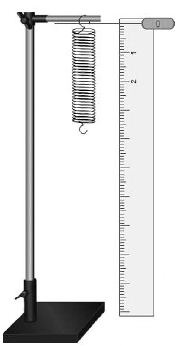
\includegraphics[scale=0.6]{Imagenes/Practica_01_04.png}
\end{figure}
\end{frame}
\begin{frame}
\frametitle{Paso 4 - Montaje experimental}
\setbeamercolor{item projected}{bg=bole,fg=white}
\setbeamertemplate{enumerate items}{%
\usebeamercolor[bg]{item projected}%
\raisebox{1.5pt}{\colorbox{bg}{\color{fg}\footnotesize\insertenumlabel}}%
}
\begin{enumerate}[<+->]
\item Coloca una pesa de \SI{50}{\gram} en el extremo del resorte y mide su estiramiento.
\item Registra los datos en la tabla de datos.
\item Repite el procedimiento anterior aumentando sucesivamente \SI{50}{\gram} al extremo del resorte, así hasta alcanzar \SI{200}{\gram}
\end{enumerate}
\end{frame}
\begin{frame}
\frametitle{Tabla de registro}
\begin{table}
\centering
\begin{tabular}{c | c | c}
Fuerza (\textbf{F}) & Estiramiento ($x$) & Constante $k = F / x$ \\ \hline
\SI{50}{\gram} & & \\ \hline
\SI{100}{\gram} & & \\ \hline
\SI{150}{\gram} & & \\ \hline
\SI{200}{\gram} & & \\ \hline
\end{tabular}
\end{table}
\end{frame}
\begin{frame}
\frametitle{Paso 5 - Montaje experimental}
Elabora una gráfica de $F$ vs $x$, \pause observa el tipo de curva obtenida.
\end{frame}

\section{Trabajo a continuar}
\frame{\tableofcontents[currentsection, hideothersubsections]}
\subsection{Marco teórico}


\begin{frame}
\frametitle{Investigación para el marco teórico}
\setbeamercolor{item projected}{bg=blue-violet,fg=white}
\setbeamertemplate{enumerate items}{%
\usebeamercolor[bg]{item projected}%
\raisebox{1.5pt}{\colorbox{bg}{\color{fg}\footnotesize\insertenumlabel}}%
}
\begin{enumerate}[<+->]
\item Define el concepto de variable dependiente y variable independiente.
\item Escribe el enunciado de la Ley de Hooke.
\item ¿Qué es la constante de un resorte?
\item Menciona y describe 3 aplicaciones de los resortes.
\end{enumerate}
\end{frame}

\section{Evaluación}
\frame{\tableofcontents[currentsection, hideothersubsections]}
\subsection{Elementos a calificar}

\begin{frame}
\frametitle{Elementos a evaluar}
\setbeamercolor{item projected}{bg=cadetgrey,fg=black}
\setbeamertemplate{enumerate items}{%
\usebeamercolor[bg]{item projected}%
\raisebox{1.5pt}{\colorbox{bg}{\color{fg}\footnotesize\insertenumlabel}}%
}
\begin{enumerate}[<+->]
\item Elaboración del marco teórico.
\item Participación en la investigación y en la consulta de bibliografía.
\seti
\end{enumerate}
\end{frame}
\begin{frame}
\frametitle{Elementos a evaluar}
\setbeamercolor{item projected}{bg=cadetgrey,fg=black}
\setbeamertemplate{enumerate items}{%
\usebeamercolor[bg]{item projected}%
\raisebox{1.5pt}{\colorbox{bg}{\color{fg}\footnotesize\insertenumlabel}}%
}
\begin{enumerate}[<+->]
\conti
\item Participación en la investigación experimental.
\item Material completo.
\item Desarrollo del experimento.
\seti
\end{enumerate}
\end{frame}
\begin{frame}
\frametitle{Elementos a evaluar}
\setbeamercolor{item projected}{bg=cadetgrey,fg=black}
\setbeamertemplate{enumerate items}{%
\usebeamercolor[bg]{item projected}%
\raisebox{1.5pt}{\colorbox{bg}{\color{fg}\footnotesize\insertenumlabel}}%
}
\begin{enumerate}[<+->]
\conti
\item Interpretación, análisis y discusión de resultados.
\item Elaboración de conclusiones.
\item Elaboración y entrega del informe de la práctica.
\end{enumerate}
\end{frame}

\section{Para la siguiente clase}
\frame{\tableofcontents[currentsection, hideothersubsections]}
\subsection{Revisión}

\begin{frame}
\frametitle{Para la siguiente clase}
\setbeamercolor{item projected}{bg=coralred,fg=white}
\setbeamertemplate{enumerate items}{%
\usebeamercolor[bg]{item projected}%
\raisebox{1.5pt}{\colorbox{bg}{\color{fg}\footnotesize\insertenumlabel}}%
}
\begin{enumerate}[<+->]
\item Presentarse con bata.
\item Subir a Teams el marco teórico.
\item Trabajo en la sesión.
\end{enumerate}
\end{frame}

\end{document}